This chapter provides detailed specifications of the system under development.

\section{Functional Requirements}

This section describes each function/feature provided by our system. These functions are logically grouped into modules based on their purposes. The users in our system are categorized as client (is able to sell), customer (is able to buy) and administrator.

\subsection*{Module 1: Registrations}
\begin{outline}
    \1 \textbf{Function 1: Register an account} \\
    The system lets users register an account on the website as a client and as a customer.
        \2 \textbf{Function 1a: Register as a client} \\
        The register form prompts the user to enter their details i.e. Name, Email, Password. The form is submitted and an unverified client account is created. The user receives a link on their email address which completes account verification.
        \2 \textbf{Function 1b: Register as a customer} \\
        The register form prompts the user to enter their details i.e. Name, Email, Password. The form is submitted and an unverified customer account is created. The user receives a link on their email address which completes account verification.
\end{outline}

\subsection*{Module 2: Buying and Selling}
\begin{outline}
    \1 \textbf{Function 1: Only client type users can upload item(s) to sell} \\
    A registered client can upload an item to sell through the mobile application. The system prompts the client for item photos, item category and item details and the item is added to the item inventory.
    \1 \textbf{Function 2: Add item to cart} \\
    A certain button on the item page prompts the system to add the item to the user's cart. All consequent item(s) added without checkout, are added to the same cart unless cleared.
    \1 \textbf{Function 3: Clear item from cart} \\
    The system allows the user to remove a previously added item from the cart. If cart is empty, the checkout link is no longer accessible.
\end{outline}

\subsection*{Module 3: Order Handling}
\begin{outline}
    \1 \textbf{Function 1: Place an order} \\
    The system allows the user to checkout when there is one or more quantity of item(s) in the cart. The checkout button prompts the system to do a user check. The next operation depends on whether the user is registered or unregistered. Once an order is placed, the client for the particular product(s) receives notifications with the order details and a suitable time-frame.
        \2 \textbf{Function 1a: Place order as a registered user} \\
        The system requests the user to enter new, or choose preexisting billing and delivery information. The order is then placed and assigned a unique order number for later use.
        \2 \textbf{Function 1b: Place order as an unregistered user} \\
        The system requests the user to register. The process in Module 1, Function 1b is carried out. This is followed by the system prompting the user for billing and delivery information. The order is then placed and assigned a unique order number for later use.
    \1 \textbf{Function 2: Cancel an existing order} \\
    The system lets a user cancel an existing order if it is not yet dispatched. The system checks the status against the order number. If it meets the case, the order is removed from the database and the client receives notifications of order cancellation.
    \1 \textbf{Function 3: The user can provide different billing and shipping addresses for an order}\\
    The system lets user decide billing and shipping addresses differently, with older ones as default selected option(s). The system stores the order such that once it is billed for, it is delivered to the recipient.
\end{outline}

\subsection*{Module 4: Delivery System}
\begin{outline}
    \1 \textbf{Function 1: Customer and client are notified of order delivery status} \\
    The client is notified of an incoming order and it is stored in their portal as an ongoing order, not yet collected. Once collected by the rider, it is confirmed as such. The admin receives the notification and is prepared to receive the order for quality assurance. Once it leaves the admin, the user is notified that the order has been dispatched and is to be expected. The user receives the order, it is confirmed by the rider, and the order delivery is complete.
\end{outline}

\subsection*{Module 5: Admin Portal}
\begin{outline}
    \1 \textbf{Function 1: Admin can remove items from the database} \\
    If a certain item does not fit the website's criteria for product, admin can remove it from the website. The client is notified that the order has been removed since it does not comply with our standards.
\end{outline}
\subsection*{Module 6: User Account Portal}
\begin{outline}
    \1 \textbf{Function 1: User can change billing and shipping information} \\
    Previous billing and shipping address can be deleted. The system removes information from its database. User can then choose to add a new set of information that is updated in our database.
    \1 \textbf{Function 2: User can change notification settings}
        \2 \textbf{Function 2a: Promotional notifications can be turned off} \\
        User notifications for promotions are sent via email. They can be turned off via the portal. User is removed from mailing list. Upon next login session user is reminded to turn on their promotional emails.
        \2 \textbf{Function 2b: Order notifications must be turned on for at least one medium} \\
        User receives order notifications through email and phone. This can be turned off through the portal, however, user must have at least one active notification medium for orders.
    \1 \textbf{Function 3: User can retrieve order history} \\
    User can access order history through account portal. The order contains details relevant to order.
\end{outline}

\subsection*{Module 7: Shop Handler}
\begin{outline}
    \1 \textbf{Function 1: Registered clients can create a shop} \\
    On account registration as a client, system responds with a page where client can create a shop. Shop handles all client data with regards to buying and selling products. The shop creation requires the client to enter a Name, Address and Phone Number. The system verifies the shop upon admin approval, and clients can then start selling.
    \1 \textbf{Function 2: Registered clients can change shop details} \\
    The client can change shop address and number through the shop portal inside their account. This cannot be done during an ongoing order on the current shop. Once all orders from the current shop are delivered, only then client can change shop details.
\end{outline}

% --- The above is to be modified as per your project, e.g. a flat list if your system has limited functional requirements.

\section{Non-functional Requirements}

\subsection*{Performance:}
\begin{outline}
    \1 Response time should not exceed 12 seconds for all pages and 7 seconds for the landing page
    \1 System should be able to handle 250 users simultaneously
    \1 50 simultaneously placed orders should be handled without crashes and errors
\end{outline}

\subsection*{Interface:}
\begin{outline}
    \1 Client should be able to upload an item to sell in 3 steps
    \1 Website and Mobile Application should have consistent color scheme
\end{outline}

\subsection*{Resource:}
\begin{outline}
    \1 Mobile Application should run without lag on 1 MB RAM smartphones
    \1 Quality Assurance requires a physical space for order handling
    \1 Quality Assurance requires personnel
\end{outline}

\subsection*{Verification:}
\begin{outline}
    \1 Email verification API should be deployed
    \1 Client has to be verified through contact before email verification
\end{outline}

\subsection*{Documentation:}
\begin{outline}
    \1 Version control maybe supplemented by proper documentation of the versions
\end{outline}

\subsection*{Security:}
\begin{outline}
    \1 User login session has to expire after 24 hours
    \1 Payment and all user information is encrypted
\end{outline}

\subsection*{Portability:}
\begin{outline}
    \1 Database backup must be maintained every 10 days
\end{outline}

\subsection*{Quality:}
\begin{outline}
    \1 Product placed on the website must have equal to or more than 3 images
    \1 Item(s) with orders more than 3 and rating less than or equal to 2.5 is reviewed
    \1 More than 90\% of user testing should be positive 
\end{outline}

\subsection*{Maintainabilty:}
\begin{outline}
    \1 New version must contain all older information
    \1 Code should allow for easy new module integrations
\end{outline}

\subsection*{Usability:}
\begin{outline}
    \1 Client survey after 2 months should have a usability score of 8/10 or more
\end{outline}

\section{External Interfaces}

\subsection{User Interfaces}
We have created an interactive dummy mobile app which is accessible through this link: https://marvelapp.com/jaefbg9/screen/62586242

\subsection{Application Program Interface (API)}
The APIs used for our system will be: 
\begin{outline}
    \1 Google Recommendations API (subject to change)
    \1 Social Login
    \1 Email Sender
    \1 User Authentication API by PassportJS
    \1 Facebook API
\end{outline}

\subsection{Hardware/Communication Interfaces}
For \textbf{Hardware Interfaces}, the Web Application would require hardware used to connect to the internet. The Mobile Application would require hardware that supports Android Operating System and internet connectivity. \\ For \textbf{Communication Interfaces}, we will be using the HTTP and TCP/IP protocol.

\section{Use Cases}
This section presents detailed use cases of our system.
\begin{figure}
  \caption{UseCase 1: Vendor Registration}
  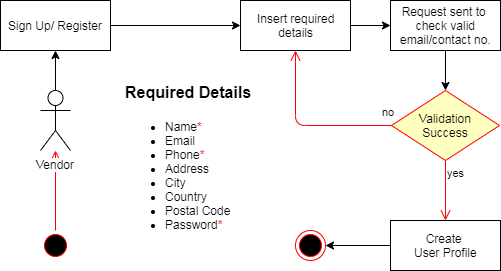
\includegraphics[width=0.75\textwidth]{Vendor_Registration.png}
  \centering
\end{figure}
\begin{figure}
  \caption{UseCase 2: How to Create a Shop}
  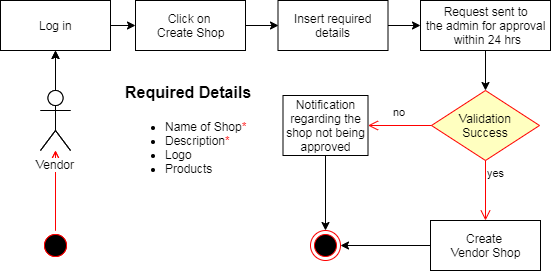
\includegraphics[width=0.75\textwidth]{Shop_Creation.png}
  \centering
\end{figure}
\begin{figure}
  \caption{UseCase 3: Upload a New Product}
  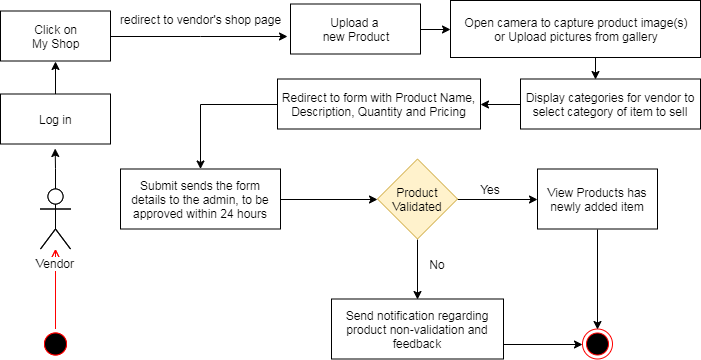
\includegraphics[width=0.75\textwidth]{UploadAProduct.png}
  \centering
\end{figure}
\begin{figure}
  \caption{UseCase 4: Edit/Update an existing Product}
  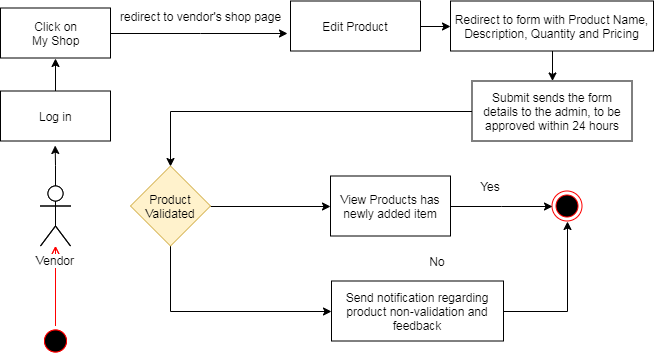
\includegraphics[width=0.75\textwidth]{EditMyProduct.png}
  \centering
\end{figure}

\section{Datasets}
This section describes the specific dataset(s) used to build our system. An appropriate snapshot of the dataset(s) is also included. Futher details, when needed, are presented in the appendix.

\section{System Diagram}
This diagram gives a high-level view of the different components of our system and the interactions between them.
The tools and technologies to be used in the system are:
\begin{outline}
    \1 HTML/CSS/Javascript, React and Bootstrap for front-end
    \1 JQuery, Nodejs, and its modules such as Expressjs and Passportjs for back-end
    \1 MongoDB for database
    \1 Amazon Web Services for hosting
    \1 React native for mobile app development
\end{outline}
The module Registration and User Account Portal will be using Passportjs extensively for user authentication, maintaining user sessions and such. The other tools and technologies will be utilized by all modules across the board.
    The system diagram for our system is placed on the next page.

\begin{figure}
  \caption{System Diagram}
  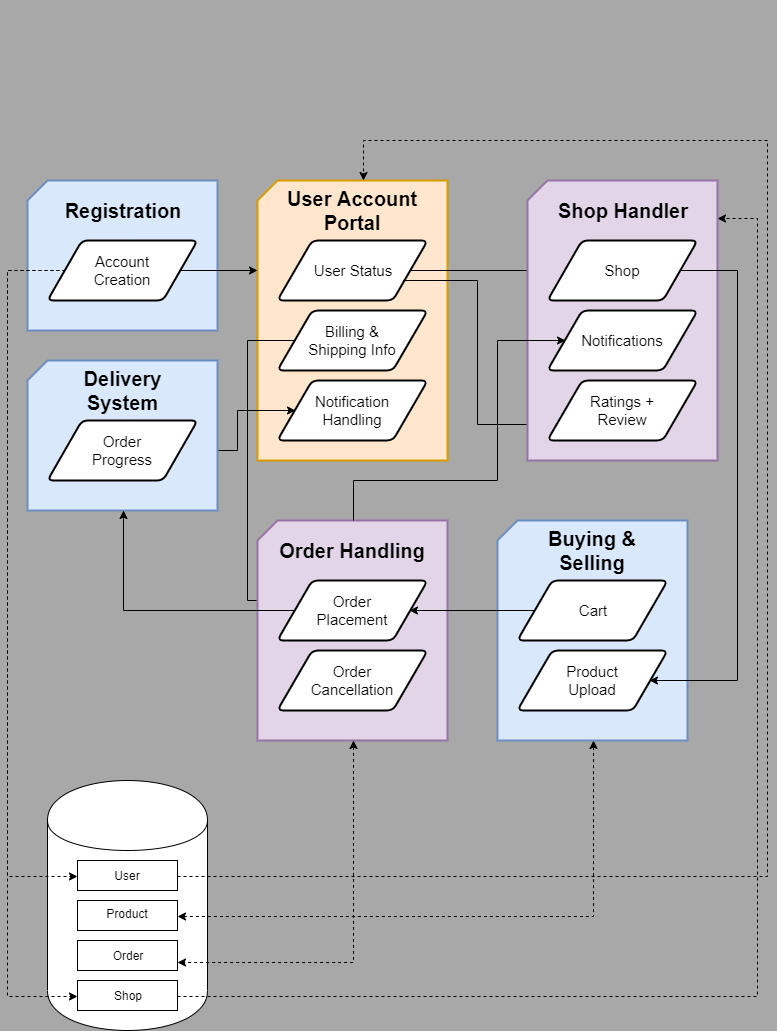
\includegraphics[width=0.75\textwidth]{System_Diagram.png}
  \centering
\end{figure}